
\chapter{Используемые технологии}
\section{Список технологий}

\hyperlink{http}{HTTP} --- это прокол передачи данных. В настоящее время существует для передачи
произвольных данных и подразумевает наличие клиента и сервера~\cite{http}.
Клиенты инициализирует запрос, а серверы – ожидают соединения для передачи
запроса, производят какие-либо действия и посылают результат обратно. Прокол
используется во Всемирной паутине для получения информации с веб-сайтов. А
также протокол используется для для транспорта других протоколов с прикладным
уровнем. Основным объектом манипуляции является ресурс, на который указывается URI.

Nginx [engine x] —-- это HTTP-сервер и обратный прокси-сервер, почтовый
прокси-сервер, а также TCP/UDP прокси-сервер общего назначения, изначально
написанный Игорем Сысоевым~\cite{nginx}.

Прокси --- сервер (proxy-server) – это особый тип приложения, которое
выступает в роли посредника между клиентскими и серверными частями
распределенных сетевых приложений. Предполагается, что клиенты принадлежат
внутренней (защищаемой) сети, а серверы – внешней (потенциально опасной).

С++ --- язык общего назначения и задуман для того, чтобы настоящие программисты получили
удовольствие от самого процесса программирования. За исключением второстепенных деталей он
содержит язык С как подмножество. Язык С расширяется введением гибких и эффективных средств,
предназначенных для построения новых типов~\cite{cpp}

Kaldi --- это набор инструментов для распознавания речи, свободно доступный по
лицензии Apache. Kaldi стремится предоставить программное обеспечение, которое
является гибким и расширяемым.~\cite{kaldi}.

CMU Sphinx --- является общим термином для описания группы систем распознавания
речи, разработанных в Университете Карнеги-Меллона. Они включают в себя серию
распознавателей речи и акустического модельного тренажера~\cite{sphinx}.

libevent --- библиотека для асинхронного уведомления о событиях со всроенным
HTTP~--~сервером.

CMake — кроcсплатформенная утилита для автоматической сборки программы из
исходного кода. При этом сама CMake непосредственно сборкой не занимается,
а представляет из себя front-end. В качестве back-end`a могут выступать
различные версии make и Ninja~\cite{cmake}.

\section{HTTP сервер}
Сервер распознавания речи речи включает в себя HTTP-сервер, с помощью которого
будет реализован внешний интерфейс приложения (\hyperlink{api}{API}), чтобы другие
подсистемы могли взаимодействовать с ASR.

Протокол HTTP --- это протокол прикладного уровня, который имеет:
\begin{enumerate}
    \item Строка запроса
    \item Заголовки
    \item Данные, отделённые от заголовков пустой строкой
\end{enumerate}

\begin{lstlisting}[caption={Общая структура HTTP протокола}, label={lst:http:struct}]
<Method> <URI> <Version>\r\n
Host: <example.com>\r\n
User-Agent: <agent>\r\n
Header1: <val1>\r\n
Header2: <val2>\r\n
...
HeaderN: <valN>\r\n
\r\n
Payload
\end{lstlisting}

В листинге~\ref{lst:http:struct} представлена общая структура протокола HTTP.
\begin{itemize}
    \item Method --- метод обращения к серверу.
    \begin{itemize}
        \item GET --- получить от сервера данные
        \item POST --- загрузить данные на сервер
        \item PUT --- изменить данные на сервере
        \item DELETE --- удалить данные на сервере
        \item MOVE --- переместить данные
    \end{itemize}
    \item URI --- строка, представляющая путь и аргументы.{\tt URI=URL?QUERY}
    \begin{itemize}
        \item URL --- строка описывающая путь (\texttt{/some/path})
        \item QUERY --- строка после знака <<\verb!?!>>, что означает наличие аргументов,
            содержащая набор ключ=значение, разделённая знаком \texttt{\&} \\
            <<\verb!key1=val1\&key2=val2\&...\&keyN=valN!>>
    \end{itemize}
    \item Versoin --- версия протокола(\texttt{HTTP/1.1} или \texttt{HTTP/1.0})
    \item Header --- имя(ключ) заголовка
    \begin{itemize}
        \item Host --- заголовок, указывающий имя сервера, к которому происходит обращение
        \item User-Agent --- заголовок, указывающий имя клиента
    \end{itemize}
    \item val --- значения соотвествующего заголовка
    \item Payload --- данные передаваемые от клиента к серверу
\end{itemize}

Также существует специальный заголвок \texttt{Transfer-Encoding}, который при
значении \texttt{chunked} позволяет сообщить, что будет происходить потоковая передача.
При такой передачи данных клиент посылает размер, в шестнадцатеричной системе
счисления, следующего куска данных, после чего отсылает данный кусок данных, и
повторяет данную процедуру необходимое число. Когда клиент закончил передачу данных,
он сообщает серверу, что следующий кусок данных содержит 0 байт.

\begin{lstlisting}[caption={Пример \texttt{Transfer-Encoding: chunked}}, label={lst:http:chunked}]
POST /path/to/file HTTP/1.1\r\n
Host: example.com\r\n
User-Agent: client\r\n
Transfer-Encoding: chunked\r\n
\r\n
a\r\n
<10 байт>\r\n
f\r\n
<15 байт>\r\n
0\r\n
\end{lstlisting}

В ином случае, когда не указан \texttt{Transfer-Encoding}, клиент должен сообщить
размер посылаемых данных в байтах с помощью заголовка \texttt{Content-Type}.

\section{Форматы аудио файлов}
Существует множество различных аудио форматов. Наиболее часто используются такие
форматы как MP3 (MPEG-2 Audio Layer III) и WAV. Тип формата обычно определяется
расширением файла (то, что идет после точки в имени файла .mp3, .wav, .ogg, .wma)~\cite{audio}.

Кодек – это определенный алгоритм кодирования и сжатия данных в аудио-формат.
Для некоторых типов файлов кодек однозначно определен. Например в формате mp3
всегда используется кодек MPEG Layer-3, а в формате mp4 могут быть использованы
разные кодеки~\cite{audio}.

Ниже представлен список используемых форматов:
\begin{itemize}
    \item \hyperlink{wav}{WAV} --– один из первых аудио-форматов. Обычно используется для хранения
    несжатых аудио-записей (PCM), идентичных по качеству звука записям на
    компакт-дисках (audio-CD). В среднем одна минута звука в формате wav занимает
    около 10 мегабайт~\cite{audio}.
    \item \hyperlink{pcm}{PCM} --- цифровое представление аналогового сигнала, в
    котором сигнал сначала дискретизируется (то есть, величина сигнала фиксируется
    в определённые интервалы времени) затем квантуется (то есть, величина сигнала
    в каждый из дискретных интервалов представляется наиболее близким значением из
    допустимых), а затем кодируется с помощью цифрового представления~\cite{pcm}.
\end{itemize}

\section{Nginx}
Данная подсистема используется для стандартизации версии протокола HTTP. По скольку
сейчас используется две версии протокола: \texttt{HTTP/1.0} и \texttt{HTTP/1.1},
между которыми существует небольшие различия. ASR реализует HTTP/1.1 версии протокола,
в которой можно держать одну TCP-сессию для нескольких запросов.

Nginx служит прокси-сервером, который позволяет абстрагироваться от того, какую
версию протокола использует клиент. Также при необходимости он может осуществлять
балансировку запросов.
\begin{lstlisting}[caption={Пример конфигурации Nginx}, label={ngx:loc:asr}]
server {
    ...
    location ~^\/(speech-recognition|asr) {
        proxy_http_version 1.1;
        proxy_request_buffering off;
        proxy_pass http://<asr_address>:<asr_port>;
    }
    ...
}
\end{lstlisting}

В листинге~\ref{ngx:loc:asr} представлен пример конфигурации Nginx для проксирования
запросов к серверу ASR. Как можно заметить при проксировании выставляется
версия протокола \texttt{HTTP/1.1}, также выключается буферизация, чтобы позволить
потоковую передачу данных на сервер распознавания.


\section{Распозавание речи}
Для распознавания речи решено использовать готовые решения.
\subsection{Kaldi}
Kaldi предоставляет современный и гибкий код, написанный на \texttt{C++}, который
легко модифицировать и расширять. Важные особенности включают в себя:

\begin{itemize}
    \item Интеграцию на уровне кода с библиотекой для конструирования, комбинирования
        и поиска взвешенных конечных преобразователей (libfst)
    \item Обширную поддержку линейной алгебры
    \item Матричную библиотеку, которая упаковывает стандартные процедуры BLAS и LAPACK.
    \item Расширяемый дизайн
    \item Алгоритмы представляют общий интерфейс, насколько это возможно
    \item Универсальные алгоритмы
\end{itemize}

Также Kaldi предоставляет готовые рецепты для построения систем распознавания речи,
которые работают из широко доступных баз данных.

Он поддерживает линейное преобразование, MMI,
усиленное MMI и MCE дискриминационное обучение, дискриминационное обучение в
пространстве признаков и глубокие нейронные сети.

\subsection{CMU Sphinx}

CMUSphinx собирает более 20 лет исследований CMU. Все преимущества сложно перечислить,
но лишь некоторые из них:
\begin{itemize}
    \item Современные алгоритмы распознавания речи для эффективного распознавания речи.
    \item Инструменты CMUSphinx разработаны специально для низкоресурсных платформ
    \item Гибкая конструкция
    \item Фокус на разработке практических приложений, а не на исследованиях
    \item Поддержка многих языков
    \item Активное сообщество
    \item Активная разработка и график выпуска
    \item Широкий спектр инструментов для многих целей, связанных с распознаванием речи
    \begin{itemize}
        \item определение ключевых слов
        \item выравнивание
        \item оценка произношения
    \end{itemize}
\end{itemize}

\chapter{ПРОЕКТИРОВАНИЕ СИСТЕМЫ}
\section{Описание работы сервера распознавания речи}
Для реализации HTTP-сервера используется библиотека \textit{libevent}, которая
предоставляет удобный интерфес.

Библиотека позволяет опустить TCP уровень и реализовывать только логику обработки
запроса. Для этого необходимо создать несколько объектов:
\begin{enumerate}
    \item event\_base~---~структура, хранящая все зарегестрированные события
    \item evhttp~---~структура http поверх event\_base, добавляющая возможность
    регистрировать HTTP событие
\end{enumerate}

Стоит отметить, что при реализации используется класс, и слудющие примеры вызываются
в методах, у которых есть доступ к приватным членам класса. Также используются
<<Resource Acquisition is Initialization>(\hyperlink{raii}{RAII})~---~
захват ресурса есть инициализация,который позволяет создать объект и указать
способ освобождения памяти при уничтожении объекта, когда он выходит за область
видимости.

В листинге~\ref{lst:class:types} представлены типы данных, уникальных указателей,
которые реализуют RAII.
\begin{lstlisting}[caption={Описание некоторых типов данных}, label={lst:class:types}]
using ptr_base = unique_ptr<event_base, decltype(&event_base_free)>;
using ptr_http = unique_ptr<evhttp, decltype(&evhttp_free)>;
\end{lstlisting}

После этого необходимо привязать event\_base к паре \texttt{ip:port}, чтобы иметь
возможность принимать соединния через сокет на заданном адресе. В листинге~\ref{lst:ev:init}
приводится пример инициализации библиотеки.

\begin{lstlisting}[caption={Пример инициализации библиотеки \textit{libevent}}, label={lst:ev:init}]
...
this->base = new ptr_base(event_base_new(), &event_base_free);
if (!base)
    KALDI_ERR << "Failed to create new base_event.";

this->http = new ptr_http(evhttp_new(base->get()), &evhttp_free);

if (!http) {
    KALDI_ERR << "Failed to create new http event";
}
auto BoundSock = evhttp_bind_socket_with_handle(http->get(), address.c_str(), port);
if (!BoundSock)

    KALDI_ERR << "Failed to bind server socket.";
if ((this->socket = evhttp_bound_socket_get_fd(BoundSock)) == -1)
    KALDI_ERR << "Failed to get server socket for next instance.";


...
\end{lstlisting}

Данная библиотека позволяет реализовать многопоточное обслуживание при заданном
количестве потоков, что позволяет не создавать новый поток на каждое соединение,
тем самым уменьшив затраты на обслуживание. Создание каждого потока происходит
последовательно. В листинге~\ref{lst:ev:thread} приводится пример создания
нескольких потоков для обслуживания. Также стоит отметить, что при создании
нового потока, ему задаётся $\lambda$~-~функция, которая будет вызвана при уничтожении
потока~---~это необходимо, что корректно освободить память при завершении программы.

\begin{lstlisting}[caption={Пример создания нескольких потоков обслуживания}, label={lst:ev:thread}]
...
ptr_base EventBase(event_base_new(), &event_base_free);
if (!EventBase)
    throw runtime_error("Failed to create new base_event.");

ptr_http EvHttp(evhttp_new(EventBase.get()), &evhttp_free);

if (!EvHttp)
    throw runtime_error("Failed to create new evhttp.");


if (evhttp_accept_socket(EvHttp.get(), socket) == -1)
    throw runtime_error("Failed to bind server socket for new instance.");


auto signal_int = evsignal_new(EventBase.get(), SIGINT, signal_cb, EventBase.get());

Threads.emplace_back(
        new thread(routine, move(EvHttp), move(EventBase), &Threads, socket, sa, signal_int),
        [signal_int](thread *t) {
            event_add(signal_int, nullptr);
            raise(SIGINT);

            t->join();

            delete t;
        });
...
\end{lstlisting}

При создании потока ему задаётся функция, которую необходимо выполнить: \texttt{routine}
, в которой происходит инициализация библиотеки для распознавания речи. В листинге~
\ref{lst:routine} представлен код, который регистрирует функции обработчика HTTP-запросов,
после чего вызывает функцию, которая будет обрабатывать новые соединения и вызывать
обработчики.

При регистрации HTTP-обработчика указывается URI, функция обратного вызова и аргументы,
также имеется общий обработчик, которые вызывается, когда нет совпадений URI.

\begin{lstlisting}[caption={Инициализация обработчиков}, label={lst:routine}]
...
evhttp_set_gencb(EvHttp.get(), callback_recognize, &sa);
event_base_dispatch(EventBase.get());
\end{lstlisting}

Реализация обработки запроса состоит из следующих пунктов:
\begin{enumerate}
    \item Прочитать необходимые Заголовки
    \item Проверить их корректность
    \item Подготовить библиотеку для распознавания
    \item Передать аудио-поток в данную библиотеку
\end{enumerate}

Для того, чтобы управлять поведением ASR введены следующие HTTP-заголовки:
\begin{itemize}
    \item SR-Key~---~Фразы, перечисленные через запятую, которые необходимо распознать
    \item Content-Type~---~формат аудио-потока.
    \begin{itemize}
        \item {\tt audio/x-wav} для wav формата
        \item {\tt audio/x-pcm} для pcm формата
    \end{itemize}
\end{itemize}

В процессе распознавание необходимо проверять наличие ключевых фраз, и при их
обнаружении возвращать ответ со статусом 200, что означает успех, а также в теле
указать распознанную фразу. Иначе вернуть 404, что означает <<ничего не найдено>>.

\section{Принцип работы системы}
В процессу работы системы IVR, ей понадобится получить ответ от собеседника,
соотвественно необходимо будет отправить аудио-поток(речь) от клиента на распознавания,
чтобы узнать ответ на заданный вопрос.

Управлением аудио-потоком занимается сервер маршрутизации аудио потоков(\hyperlink{msr}{MSR}).
Его задачей является перенаправлять аудио-поток от источника в заданные подсистемы.
MSR умеет работать со следующими системами:
\begin{itemize}
    \item Система распознавания речи
    \item Запись разговора
    \item Синтез речи
    \item WebDav~---~ протокол передачи данных поверх HTTP
\end{itemize}

Рассмотрим пример схемы связей подсистем~\ref{fig:schema}\footnote{Элемент системы
\texttt{CORE}~---~выполняет роль маршрутизации звонков и не рассматривается, а лишь
дополняет схему} на примере
системы автообзвонщика~---~ необходимо обзвонить всех клиентов, у которых имеется
задолженность и сообщить её, при этом:
\begin{enumerate}
    \item Представиться
    \item Уточнить имя клиента на случай, если номер принадлежит другому
    \item Уточнить адрес проживания
    \item Сообщить сумму
    \item Узнать о платёжеспособности
\end{enumerate}

\begin{figure}[h!]
    \centering
    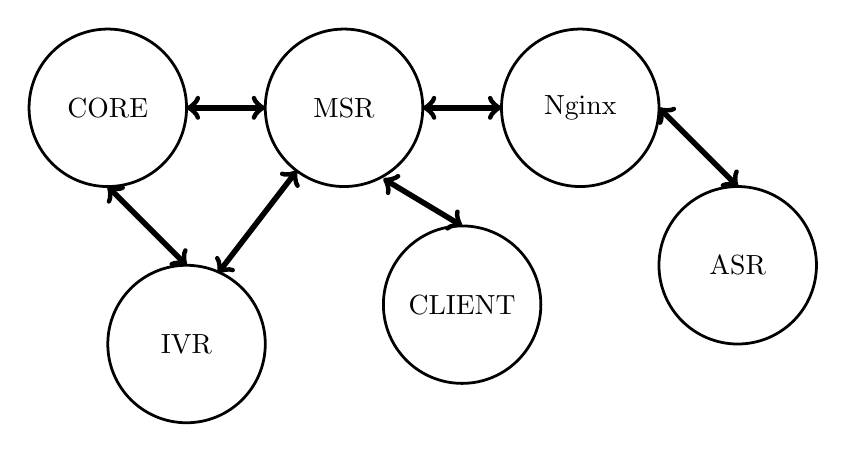
\begin{tikzpicture}
        \draw[line width=1](6,1) circle(1) node {ASR} +(1,-1);
        \draw[line width=2,<->] (6, 2) -- +(-1, 1);
        \draw[line width=1](4,3) circle(1) node {Nginx} +(1,-1);
        \draw[line width=1](2.5,0.5) circle(1) node {CLIENT} +(1,-1);
        \draw[line width=2,<->] (2.5, 1.5) -- +(-1,0.6);
        \draw[line width=1](1,3) circle(1) node {MSR} +(1,-1);
        \draw[line width=2,<->] (2,3) -- +(1,0);
        \draw[line width=2,<->] (-0.6,0.9) -- +(1,1.3);
        \draw[line width=1](-1,0) circle(1) node {IVR} +(1,-1);
        \draw[line width=2,<->] (-1,3) -- +(1,0);
        \draw[line width=1](-2,3) circle(1) node {CORE} +(1,-1);
        \draw[line width=2,<->] (-2,2) -- +(1,-1);
    \end{tikzpicture}
    \caption{Схема связи подсистем}
    \label{fig:schema}
\end{figure}

Как видно на графе связей~\ref{fig:schema} все манипуляции с ASR происходят через
MSR. Система MSR и IVR общаются по протоколу HTTP через прокси-сервер Nginx.

В ходе общения системы IVR и клиента, система задаёт вопросы и сообщает фразы,
которые ожидает услышать от клиента. Для того, чтобы сообщить системе ASR какие
фразы являются ключевыми, система MSR сообщает ей в заголовке \texttt{SR-Key},
например \texttt{SR-Key: конечно, да, может быть, нет}.

После чего система MSR отправаляет аудио-поток, при этом заполняя заголовок
\texttt{Content-Type} соотвествующим значением: \texttt{audio/x-wav} или
\texttt{audio/x-pcm}, в зависимости от настроек системы.

Далее происходит процесс распознавания речи и поиска ключевых слов. При обнаружении
ключевого слово система ASR возвращает ответ со статусом 200, в тело которого
вложено распознанное ключевое слово, иначе возвращается ответ со статусом 404.
